\begin{SCn}

\scnsectionheader{\currentname}

\scnstartsubstruct

\scnheader{Предметная область чисел и числовых структур}
\scniselement{предметная область}
\scnsdmainclasssingle{число}
\scnsdclass{натуральное число;целое число;рациональное число;иррациональное число;действительное число;комплексное число;отрицательное число;положительное число;арифметическое выражение;арифметическая операция;Число Пи;Число нуль;Число один;Мнимая единица;числовая структура;система счисления;десятичная система счисления;двоичная система счисления;шестнадцатеричная система счисления}
\scnsdrelation{противоположные числа*;модуль*;сумма*;произведение*;возведение в степень*;больше*;равенство*;больше или равно*}

\scnheader{число}
\scnidtf{множество чисел}
\scnexplanation{\textbf{\textit{число}} – это основное понятие математики, используемое для количественной характеристики, сравнения, нумерации объектов и их частей. Письменными знаками для обозначения чисел служат цифры, а также символы математических операций.}

\scnheader{натуральное число}
\scnidtf{множество натуральных чисел}
\scnexplanation{\textbf{\textit{натуральное число}} – это подмножество множества \textit{целых чисел}, которые используются при счете предметов.}
\scnsubset{целое число}

\scnheader{целое число}
\scnidtf{множество целых чисел}
\scnexplanation{\textbf{\textit{целое число}} – это подмножество множества \textit{рациональных чисел}, получаемых объединением \textit{натуральных чисел} с множеством чисел, \textit{противоположных* натуральным} и \textit{нулём}.}
\scnsubset{рациональное число}

\scnheader{рациональное число}
\scnidtf{множество рациональных чисел}
\scnexplanation{\textbf{\textit{рациональное число}} – это число, представляемое обыкновенной дробью, где числитель — \textit{целое число}, а знаменатель — \textit{натуральное число}.}
\scnsubset{вещественное число}

\scnheader{иррациональное число}
\scnidtf{множество иррациональных чисел}
\scnexplanation{\textbf{\textit{иррациональное число}} – это \textit{вещественное число}, которое не является рациональным, то есть не может быть представлено в виде дроби, где числитель — \textit{целое число}, знаменатель — \textit{натуральное число}. Любое \textbf{\textit{иррациональное число}} может быть представлено в виде бесконечной непериодической десятичной дроби.}
\scnsubset{вещественное число}

\scnheader{действительное число}
\scnidtf{вещественное число}
\scnidtf{множество вещественных чисел}
\scnreltoset{объединение}{рациональное число;иррациональное число}
\scnreltoset{разбиение}{положительное число;отрицательное число;$\{$Число нуль$\}$}
\scnexplanation{\textbf{\textit{действительное число}} – это множество чисел, получаемое в результате объединения иррациональных и \textit{рациональных чисел}.}
\scnsubset{комплексное число}

\scnheader{комплексное число}
\scnidtf{множество комплексных чисел}
\scnexplanation{\textbf{\textit{комплексное число}} – число вида \textit{z=a+b*i}, где \textit{a} и \textit{b} – \textit{вещественные числа}, \textit{i} – \textit{Мнимая единица}.}

\scnheader{отрицательное число}
\scnidtf{множество отрицательных чисел}
\scnexplanation{\textbf{\textit{отрицательное число}} – число \textit{меньше*} нуля.}

\scnheader{положительное число}
\scnidtf{множество положительных чисел}
\scnexplanation{\textbf{\textit{положительное число}} – число \textit{больше*} нуля.}

\scnheader{противоположные числа*}
\scniselement{бинарное отношение}
\scnexplanation{\textbf{\textit{противоположные числа*}} – \textit{отношение}, связывающее два числа, одно из которых является \textit{отрицательным числом}, второе – \textit{положительным}, при этом \textit{модули*} этих чисел \textit{равны*}.}

\scnheader{модуль*}
\scnidtf{модуль числа*}
\scniselement{бинарное отношение}
\scnexplanation{Связки отношения \textbf{\textit{модуль*}} связывают некоторое \textit{число} (которое может быть как \textit{отрицательным}, так и \textit{положительным}) и другое \textit{число} (всегда \textit{положительное}), которое выражает расстояние от указанного числа до \textit{Числа нуль} в единицах.}

\scnheader{арифметическое выражение}
\scnidtf{множество арифметических выражений}
\scnexplanation{Каждое \textbf{\textit{арифметическое выражение}} представляет собой \textit{связку}, компонентами которой являются \textit{числа} или множества \textit{чисел}.}

\scnheader{арифметическая операция}
\scnidtf{множество арифметических операций}
\scnrelto{семейство подмножеств}{арифметическое выражение}
\scnexplanation{Каждая \textbf{\textit{арифметическая операция}} представляет собой \textit{отношение}, элементами которого являются \textit{арифметические выражения}, то есть множество \textit{арифметических выражений} какого-либо одного вида.}

\scnheader{сумма*}
\scnidtf{сложение*}
\scniselement{арифметическая операция}
\scniselement{квазибинарное отношение}
\scnexplanation{\textbf{\textit{сумма*}} – это арифметическая операция, в результате которой по данным числам (слагаемым) находится новое число (сумма), обозначающее столько единиц, сколько их содержится во всех слагаемых.

Первым компонентом связки отношения \textbf{\textit{сумма*}} является \textit{множество чисел} (слагаемых), содержащее два или более элемента, вторым компонентом – \textit{число}, являющееся результатом сложения.

Отдельно отметим, что каждая связка отношения \textbf{\textit{сумма*}} вида a = b+c может также трактоваться и как запись о вычитании чисел, например b = a-c, в связи с чем \textit{арифметическая операция} разности чисел отдельно не вводится.}
\scnrelfrom{описание типичного экземпляра}{
\scnfilelong{
\begin{figure}[H]
\centering
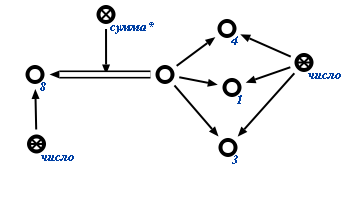
\includegraphics[width=0.8\linewidth]{figures/sd_numbers/sum.png}
\end{figure}
}}

\scnheader{произведение*}
\scnidtf{умножение*}
\scniselement{арифметическая операция}
\scniselement{квазибинарное отношение}
\scnexplanation{\textbf{\textit{произведение*}} – это \textit{арифметическая операция}, в результате которой один аргумент складывается столько раз, сколько показывает другой, затем результат складывается столько раз, сколько показывает третий и т.д.

Первым компонентом связки отношения \textbf{\textit{произведение*}} является \textit{множество чисел} (множителей), содержащее два или более элемента, вторым компонентом – \textit{число}, являющееся результатом произведения.

Отдельно отметим, что каждая связка отношения \textbf{\textit{произведение*}} вида a = b*c может также трактоваться и как запись о делении чисел, например b = a/c, в связи с чем \textit{арифметическая операция} деления чисел отдельно не вводится.}
\scnrelfrom{описание типичного экземпляра}{
\scnfilelong{
\begin{figure}[H]
\centering
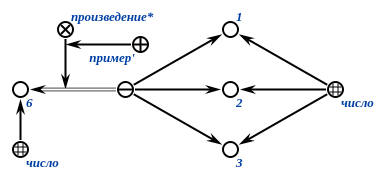
\includegraphics[width=0.8\linewidth]{figures/sd_numbers/multiplication.png}
\end{figure}
}}

\scnheader{возведение в степень*}
\scniselement{арифметическая операция}
\scniselement{бинарное отношение}
\scnexplanation{\textbf{\textit{возведение в степень*}} – это \textit{арифметическая операция}, в результате которой число, называемое основанием степени, умножается само на себя столько раз, каков показатель степени.

Первым компонентом связки отношения \textbf{\textit{возведение в степень*}} является ориентированная пара, первым компонентом которой является \textit{число}, которое является основанием степени, вторым – \textit{число}, которое является показателем степени; Вторым компонентом связки отношения \textbf{\textit{возведение в степень*}} является \textit{число}, которое является результатом возведения в степень.

Отдельно отметим, что каждая связка отношения \textbf{\textit{возведение в степень*}} вида a = $b^c$ может также трактоваться и как запись об извлечении корня или взятии логарифма, в связи с чем \textit{арифметические операции} извлечения корня и взятия логарифма отдельно не вводится.}
\scnrelfrom{описание типичного экземпляра}{
\scnfilelong{
\begin{figure}[H]
\centering
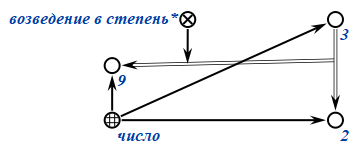
\includegraphics[width=0.5\linewidth]{figures/sd_numbers/pow.png}
\end{figure}
}}

\scnheader{больше*}
\scniselement{арифметическая операция}
\scniselement{бинарное отношение}
\scniselement{отношение строгого порядка}
\scnexplanation{\textbf{\textit{больше*}} – это \textit{арифметическая операция} сравнения чисел. Из двух чисел на координатной прямой больше то, которое расположено правее. Соответственно, первым компонентом связки \textit{отношения} \textbf{\textit{больше*}} является большее из двух \textit{чисел}.}
\scnrelfrom{описание типичного экземпляра}{
\scnfilelong{
\begin{figure}[H]
\centering
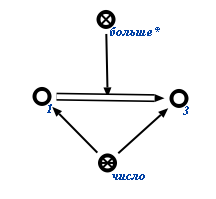
\includegraphics[width=0.5\linewidth]{figures/sd_numbers/more.png}
\end{figure}
}}

\scnheader{равенство*}
\scnidtf{равенство чисел*}
\scniselement{арифметическая операция}
\scniselement{бинарное отношение}
\scniselement{симметричное отношение}
\scniselement{рефлексивное отношение}
\scniselement{транзитивное отношение}
\scnexplanation{\textbf{\textit{равенство*}} – отношение взаимной заменяемости \textit{чисел}, которые именно в силу этой заменяемости и считаются равными. Равные \textit{числа} на числовой прямой совпадают.}
\scnrelfrom{описание типичного экземпляра}{
\scnfilelong{
\begin{figure}[H]
\centering
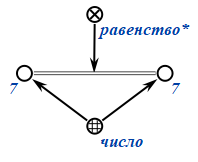
\includegraphics[width=0.5\linewidth]{figures/sd_numbers/equality.png}
\end{figure}
}}

\scnheader{больше или равно*}
\scniselement{арифметическая операция}
\scniselement{бинарное отношение}
\scniselement{отношение нестрогого порядка}
\scnexplanation{\textbf{\textit{больше или равно*}} – это \textit{арифметическая операция} сравнения чисел, при которой первое \textit{число} (первый компонент связки) может быть \textit{больше*} второго или \textit{равняться*} ему.}
\scnrelfrom{описание типичного экземпляра}{
\scnfilelong{
\begin{figure}[H]
\centering
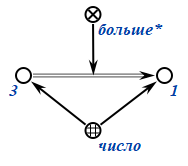
\includegraphics[width=0.5\linewidth]{figures/sd_numbers/more_or_equal.png}
\end{figure}
}}

\scnheader{Число Пи}
\scniselement{иррациональное число}
\scnexplanation{\textbf{\textit{Число Пи}} – это  математическая константа, равная отношению длины окружности к длине её диаметра.}

\scnheader{Число нуль}
\scnidtf{0}
\scniselement{целое число}
\scnexplanation{\textbf{\textit{Число нуль}} – это \textit{целое число}, разделяющее на числовой прямой \textit{положительные числа} и \textit{отрицательные числа}.}

\scnheader{Число один}
\scnidtf{1}
\scniselement{целое число}
\scniselement{натуральное число}
\scnexplanation{\textbf{\textit{Число один}} – это наименьшее \textit{натуральное число}.}

\scnheader{Мнимая единица}
\scnidtf{i}
\scniselement{комплексное число}
\scnexplanation{\textbf{\textit{Мнимая единица}} – это \textit{число}, при возведении которого в степень 2 результатом будет число, противоположное \textit{Числу один}.}

\scnheader{числовая структура}
\scnsubset{структура}
\scnexplanation{\textbf{\textit{числовая структура}} – \textit{структура}, в состав которой входят знаки \textit{арифметических выражений}, а также знаки их элементов и связи между выражениями и их элементами.}

\scnheader{система счисления}
\scniselement{параметр}
\scnexplanation{Каждая \textbf{\textit{система счисления}} представляет собой класс синтаксически эквивалентных файлов, хранимых в sc-памяти, каждый из которых может являться идентификатором какого-либо \textit{числа}.

Каждая \textbf{\textit{система счисления}} характеризуется алфавитом, т.е. конечным множеством символов (цифр), которые допускается использовать при построении файлов принадлежащих данной \textbf{\textit{системе счисления}}.}

\scnheader{десятичная система счисления}
\scniselement{система счисления}

\scnheader{двоичная система счисления}
\scniselement{система счисления}

\scnheader{шестнадцатеричная система счисления}
\scniselement{система счисления}

\scnendstruct

\end{SCn}